% Options for packages loaded elsewhere
\PassOptionsToPackage{unicode}{hyperref}
\PassOptionsToPackage{hyphens}{url}
%
\documentclass[
  12pt,
]{article}
\title{Insert title of project here}
\usepackage{etoolbox}
\makeatletter
\providecommand{\subtitle}[1]{% add subtitle to \maketitle
  \apptocmd{\@title}{\par {\large #1 \par}}{}{}
}
\makeatother
\subtitle{\url{https://github.com/maggieoshea/OSheaPearceSanchez_ENV872_EDA_FinalProject.git}}
\author{Maggie O'Shea, Garrett Pearce, and Diane Sanchez}
\date{}

\usepackage{amsmath,amssymb}
\usepackage{lmodern}
\usepackage{iftex}
\ifPDFTeX
  \usepackage[T1]{fontenc}
  \usepackage[utf8]{inputenc}
  \usepackage{textcomp} % provide euro and other symbols
\else % if luatex or xetex
  \usepackage{unicode-math}
  \defaultfontfeatures{Scale=MatchLowercase}
  \defaultfontfeatures[\rmfamily]{Ligatures=TeX,Scale=1}
  \setmainfont[]{Times New Roman}
\fi
% Use upquote if available, for straight quotes in verbatim environments
\IfFileExists{upquote.sty}{\usepackage{upquote}}{}
\IfFileExists{microtype.sty}{% use microtype if available
  \usepackage[]{microtype}
  \UseMicrotypeSet[protrusion]{basicmath} % disable protrusion for tt fonts
}{}
\makeatletter
\@ifundefined{KOMAClassName}{% if non-KOMA class
  \IfFileExists{parskip.sty}{%
    \usepackage{parskip}
  }{% else
    \setlength{\parindent}{0pt}
    \setlength{\parskip}{6pt plus 2pt minus 1pt}}
}{% if KOMA class
  \KOMAoptions{parskip=half}}
\makeatother
\usepackage{xcolor}
\IfFileExists{xurl.sty}{\usepackage{xurl}}{} % add URL line breaks if available
\IfFileExists{bookmark.sty}{\usepackage{bookmark}}{\usepackage{hyperref}}
\hypersetup{
  pdftitle={Insert title of project here},
  pdfauthor={Maggie O'Shea, Garrett Pearce, and Diane Sanchez},
  hidelinks,
  pdfcreator={LaTeX via pandoc}}
\urlstyle{same} % disable monospaced font for URLs
\usepackage[margin=2.54cm]{geometry}
\usepackage{color}
\usepackage{fancyvrb}
\newcommand{\VerbBar}{|}
\newcommand{\VERB}{\Verb[commandchars=\\\{\}]}
\DefineVerbatimEnvironment{Highlighting}{Verbatim}{commandchars=\\\{\}}
% Add ',fontsize=\small' for more characters per line
\usepackage{framed}
\definecolor{shadecolor}{RGB}{248,248,248}
\newenvironment{Shaded}{\begin{snugshade}}{\end{snugshade}}
\newcommand{\AlertTok}[1]{\textcolor[rgb]{0.94,0.16,0.16}{#1}}
\newcommand{\AnnotationTok}[1]{\textcolor[rgb]{0.56,0.35,0.01}{\textbf{\textit{#1}}}}
\newcommand{\AttributeTok}[1]{\textcolor[rgb]{0.77,0.63,0.00}{#1}}
\newcommand{\BaseNTok}[1]{\textcolor[rgb]{0.00,0.00,0.81}{#1}}
\newcommand{\BuiltInTok}[1]{#1}
\newcommand{\CharTok}[1]{\textcolor[rgb]{0.31,0.60,0.02}{#1}}
\newcommand{\CommentTok}[1]{\textcolor[rgb]{0.56,0.35,0.01}{\textit{#1}}}
\newcommand{\CommentVarTok}[1]{\textcolor[rgb]{0.56,0.35,0.01}{\textbf{\textit{#1}}}}
\newcommand{\ConstantTok}[1]{\textcolor[rgb]{0.00,0.00,0.00}{#1}}
\newcommand{\ControlFlowTok}[1]{\textcolor[rgb]{0.13,0.29,0.53}{\textbf{#1}}}
\newcommand{\DataTypeTok}[1]{\textcolor[rgb]{0.13,0.29,0.53}{#1}}
\newcommand{\DecValTok}[1]{\textcolor[rgb]{0.00,0.00,0.81}{#1}}
\newcommand{\DocumentationTok}[1]{\textcolor[rgb]{0.56,0.35,0.01}{\textbf{\textit{#1}}}}
\newcommand{\ErrorTok}[1]{\textcolor[rgb]{0.64,0.00,0.00}{\textbf{#1}}}
\newcommand{\ExtensionTok}[1]{#1}
\newcommand{\FloatTok}[1]{\textcolor[rgb]{0.00,0.00,0.81}{#1}}
\newcommand{\FunctionTok}[1]{\textcolor[rgb]{0.00,0.00,0.00}{#1}}
\newcommand{\ImportTok}[1]{#1}
\newcommand{\InformationTok}[1]{\textcolor[rgb]{0.56,0.35,0.01}{\textbf{\textit{#1}}}}
\newcommand{\KeywordTok}[1]{\textcolor[rgb]{0.13,0.29,0.53}{\textbf{#1}}}
\newcommand{\NormalTok}[1]{#1}
\newcommand{\OperatorTok}[1]{\textcolor[rgb]{0.81,0.36,0.00}{\textbf{#1}}}
\newcommand{\OtherTok}[1]{\textcolor[rgb]{0.56,0.35,0.01}{#1}}
\newcommand{\PreprocessorTok}[1]{\textcolor[rgb]{0.56,0.35,0.01}{\textit{#1}}}
\newcommand{\RegionMarkerTok}[1]{#1}
\newcommand{\SpecialCharTok}[1]{\textcolor[rgb]{0.00,0.00,0.00}{#1}}
\newcommand{\SpecialStringTok}[1]{\textcolor[rgb]{0.31,0.60,0.02}{#1}}
\newcommand{\StringTok}[1]{\textcolor[rgb]{0.31,0.60,0.02}{#1}}
\newcommand{\VariableTok}[1]{\textcolor[rgb]{0.00,0.00,0.00}{#1}}
\newcommand{\VerbatimStringTok}[1]{\textcolor[rgb]{0.31,0.60,0.02}{#1}}
\newcommand{\WarningTok}[1]{\textcolor[rgb]{0.56,0.35,0.01}{\textbf{\textit{#1}}}}
\usepackage{graphicx}
\makeatletter
\def\maxwidth{\ifdim\Gin@nat@width>\linewidth\linewidth\else\Gin@nat@width\fi}
\def\maxheight{\ifdim\Gin@nat@height>\textheight\textheight\else\Gin@nat@height\fi}
\makeatother
% Scale images if necessary, so that they will not overflow the page
% margins by default, and it is still possible to overwrite the defaults
% using explicit options in \includegraphics[width, height, ...]{}
\setkeys{Gin}{width=\maxwidth,height=\maxheight,keepaspectratio}
% Set default figure placement to htbp
\makeatletter
\def\fps@figure{htbp}
\makeatother
\setlength{\emergencystretch}{3em} % prevent overfull lines
\providecommand{\tightlist}{%
  \setlength{\itemsep}{0pt}\setlength{\parskip}{0pt}}
\setcounter{secnumdepth}{5}
\ifLuaTeX
  \usepackage{selnolig}  % disable illegal ligatures
\fi

\begin{document}
\maketitle

\#Notes to self : * Don't forget to add figure captions to exploratory
analysis

\newpage
\tableofcontents 
\newpage
\listoftables 
\newpage
\listoffigures 
\newpage

\hypertarget{rationale-and-research-questions}{%
\subsection{Rationale and Research
Questions}\label{rationale-and-research-questions}}

Extreme weather events and natural disasters seem to be on the rise
worldwide, and climate adaptation is vital to communities at risk. In
the U.S., flooding is the most common natural disaster with the cost of
flooding in the United States in 2020 estimated at \$32.1 billion (IDMC
2019, Lindsey 2022, Wing et al.~2022). These costs, both financial as
well as social, are expected to only rise as there is a predicted 24\%
increase in flooding by 2050 (Wing et al.~2022). Already, regions in the
United States are seeing drastic increases in flooding since the 1950s -
a study by the United States Environmental Protection Agency on 33 sites
around the United States found flooding to be at least five times more
common in over half the areas studies, with a strong concentration in
sites along the eastern seaboard (EPA 2022). Given the rapid increase in
flooding around the United States as well as the severe impacts this
hazard can have, adaptation is becoming increasingly important and
resources that already exist for these efforts are likely to become more
strained.

It will be increasingly important to understand the resources that are
already available to communities, the accessibility of these resources,
as well as how they are being used. This analysis seeks to uncover some
of this through examining the trends in flood mitigation assistance
provided by the Federal Emergency Management Agency. A time series
analysis helped to identify possible trends in the number of grants
received for flooding over time as well as the amount paid by FEMA to
understand if trends in the use of these resources are similarly
increasing as flooding has been. Furthermore, due to the drastic impacts
of flooding that are only increasing, we were interested to examine if
individuals are relying more heavily on ex-situ adaptation measures to
move away from these hazards, or if communities are attempting to stay
where they are despite the flooding and thus relying on in-situ
adaptation measures. The research questions that guided this work were:

\begin{enumerate}
\def\labelenumi{\arabic{enumi}.}
\tightlist
\item
  Are there trends in the number of properties that received grants to
  adapt to flooding in the United States over time?
\item
  Are there trends in the amount FEMA paid for hazard mitigation for
  flooding over time?
\item
  How do these trends differ for in-situ vs ex-situ adaptation?
\end{enumerate}

The temporal scale of the research was defined by the FEMA Mitigated
Properties dataset which included information on grants from 1985 until
2020 allowing the time series analysis to cover a 35 year time-frame.
The grants included those received in all states in the United States.
This analysis also included a brief spatial analysis focusing on one
state in particular to spatially visualize the data as well as examine
potential spatial trends in ex-situ vs.~in-situ adaptation funding.

\newpage

\hypertarget{dataset-information}{%
\subsection{Dataset Information}\label{dataset-information}}

\hypertarget{dataset-background-and-retrieval}{%
\section{Dataset Background and
Retrieval:}\label{dataset-background-and-retrieval}}

We used data managed by the Federal Emergency Management Agency's
National Emergency Management Information Systems, downloaded directly
in a CSV format through FEMA's OpenFEMA resource. The dataset includes
the record of properties that received grant assistance for hazard
mitigation through any of the Hazard Mitigation Assistance grant
programs, programs administered by FEMA that seek to reduce losses from
disasters as well as protect life and property in the face of hazards
(FEMA n.d.). This includes: the Hazard Mitigation Grant Program, the
Flood Mitigation Assistance Grant Program, and the Pre-Disaster
Mitigation Grant Program (ibid.). Entries prior to 2012 also include
grants received through the Repetitive Flood Claims Grant program and
Severe Repetitive Loss Grant Program which both were eliminated through
the Biggert Water Flood Insurance Reform Act of 2012 (ibid.). Each entry
includes data such as the total amount paid, the number of properties
receiving support, the hazard that the grant is adapting against, the
program year, and others.

For the spatial analysis, the county boundaries for North Carolina were
downloaded from the OpenESRI platform which had the State of North
Carolina's Emergency Management Agency's best current available data as
of 2020. These boundaries were identified through sources including the
North Carolina Geodetic Survey, the North Carolina Department of
Transportation, the United States Geological Survey, as well as field
surveys that have been recorded by the respective county (ArcGIS Hub
2020).

\hypertarget{data-wrangling}{%
\section{Data Wrangling}\label{data-wrangling}}

The mitigated properties dataset required three different types of
wrangling for the analysis. First, we wrangled the data to result in a
dataset with the total number of properties that received a grant for
any type of flooding adaptation and the total amount paid for these per
year. Second, we wrangled the data to have this same information, number
of properties and total amount paid, for ex-situ adaptation, or buyouts,
per year and did the same for in-situ adaptation. Finally, we wrangled
the mitigated properties dataset in the same ways - finding number of
properties and total amount paid for all flooding grants, ex-situ
grants, and in-situ grants but instead of summarizing per year, we
selected for only North Carolina grants and grouped the data by county
for our spatial analysis.

\textbf{MAKE A TABLE for type codes}

In order to do so, we first examined and explored the dataset and found
that some entries had a total amount paid that was negative. Because the
OpenFEMA information page included a note that these were manually
entered data and subject to human error, we made the assumption that
this was due to human error and removed these negative values from our
analysis. After doing so, we used this cleaned mitigated properties
dataset to create our three different types of wrangled datasets. This
involved, first, examining the ``type'' codes to identify which type
codes indicate that the grants were used for flooding. Table 1 shows the
type codes that were used, grouped by ex-situ and in-situ codes. These
type codes together were used to find all flooding grants regardless of
adaptation type.

After selecting out the relevant flooding type codes, we grouped by year
or county and summarized the datasets to find the sum of the number of
properties and the total amount paid for each category we were examining
in this analysis (amount paid for all flooding grants per year, amount
paid for ex-situ grants per year, etc.).For the total amount paid
categories specifically, using the ``priceR'' package, we adjusted each
of the total amount paid values per year for all adaptation, ex-situ,
and in-situ for inflation. Summary statistics for the respective
wrangled datasets can be found in table 2.

\newpage

\hypertarget{exploratory-analysis}{%
\subsection{Exploratory Analysis}\label{exploratory-analysis}}

After wrangling the data, we explored the data both over time as well as
totals for the number of properties and amount paid in our dataset,
compared between all flooding and ex-situ vs.~in-situ. Figure 1 shows
the differences in the total number of properties between 1985 and 2020
that received adaptation flooding, comparing all of the properties with
ex-situ and in-situ. The graph shows that more properties received
ex-situ than in-situ grants by a considerable amount.

\begin{Shaded}
\begin{Highlighting}[]
\FunctionTok{ggplot}\NormalTok{(}\AttributeTok{data =}\NormalTok{ totalprops\_pivot, }\FunctionTok{aes}\NormalTok{(}\AttributeTok{x =}\NormalTok{ Category, }\AttributeTok{y =}\NormalTok{ Total)) }\SpecialCharTok{+}
  \FunctionTok{geom\_bar}\NormalTok{(}\AttributeTok{stat =} \StringTok{"identity"}\NormalTok{, }\AttributeTok{fill =} \StringTok{"lightblue4"}\NormalTok{)}\SpecialCharTok{+}
  \FunctionTok{labs}\NormalTok{( }
    \AttributeTok{title =} \StringTok{"Total Properties Receiving Flooding Adaptation Funding from 1985 {-} 2020"}\NormalTok{, }
    \AttributeTok{x =} \StringTok{"Adaptation Type"}\NormalTok{, }
    \AttributeTok{y =} \StringTok{"Number of Properties"}\NormalTok{)}
\end{Highlighting}
\end{Shaded}

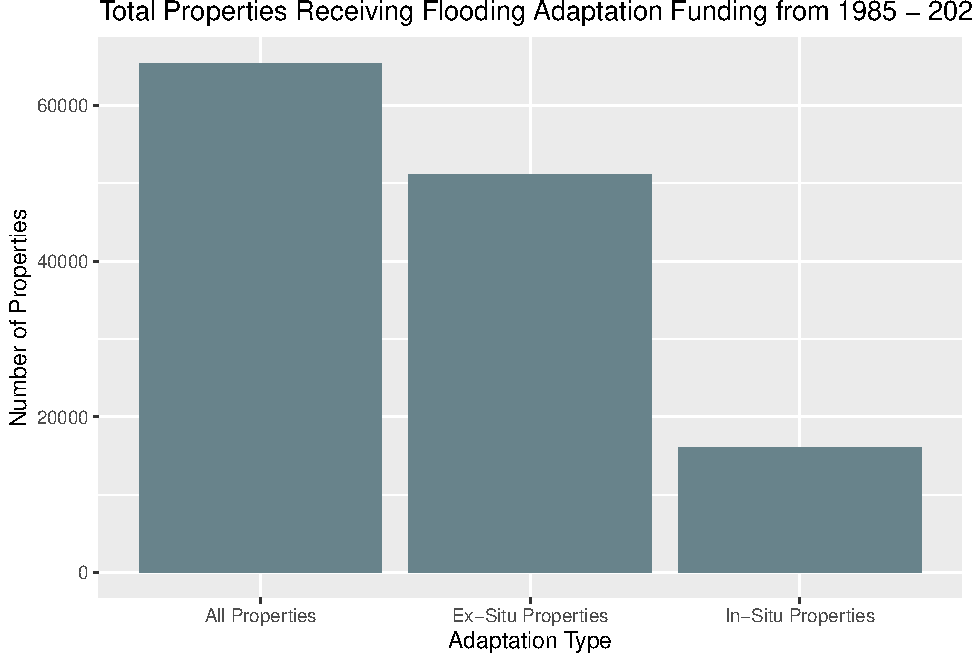
\includegraphics{finalreport_files/figure-latex/unnamed-chunk-1-1.pdf}

To examine this relationship further, we compared the total amount paid
for all adaptation types and in-situ vs.~ex-situ in Figure 2. In
including both the total amount paid as reported by FEMA as well as
these values adjusted to 2020 dollars, this figure helps to also show
the difference that inflation makes in the resulting total amount paid.

\begin{Shaded}
\begin{Highlighting}[]
\FunctionTok{ggplot}\NormalTok{(}\AttributeTok{data =}\NormalTok{ totals\_inflation\_pivot, }\FunctionTok{aes}\NormalTok{(}\AttributeTok{x =}\NormalTok{ Category, }\AttributeTok{y =}\NormalTok{ Total)) }\SpecialCharTok{+}
  \FunctionTok{geom\_bar}\NormalTok{(}\AttributeTok{stat =} \StringTok{"identity"}\NormalTok{, }\AttributeTok{fill =} \StringTok{"lightblue3"}\NormalTok{)}\SpecialCharTok{+}
  \FunctionTok{labs}\NormalTok{( }
    \AttributeTok{title =} \StringTok{"Total Amount Paid for Flooding Adaptation from 1985 {-} 2020"}\NormalTok{, }
    \AttributeTok{subtitle =} \StringTok{"Amount Paid With and Without Inflation Adjustments to 2020 USD"}\NormalTok{,}
    \AttributeTok{x =} \StringTok{"Adaptation Type"}\NormalTok{, }
    \AttributeTok{y =} \StringTok{"Amount Paid (USD)"}\NormalTok{)}
\end{Highlighting}
\end{Shaded}

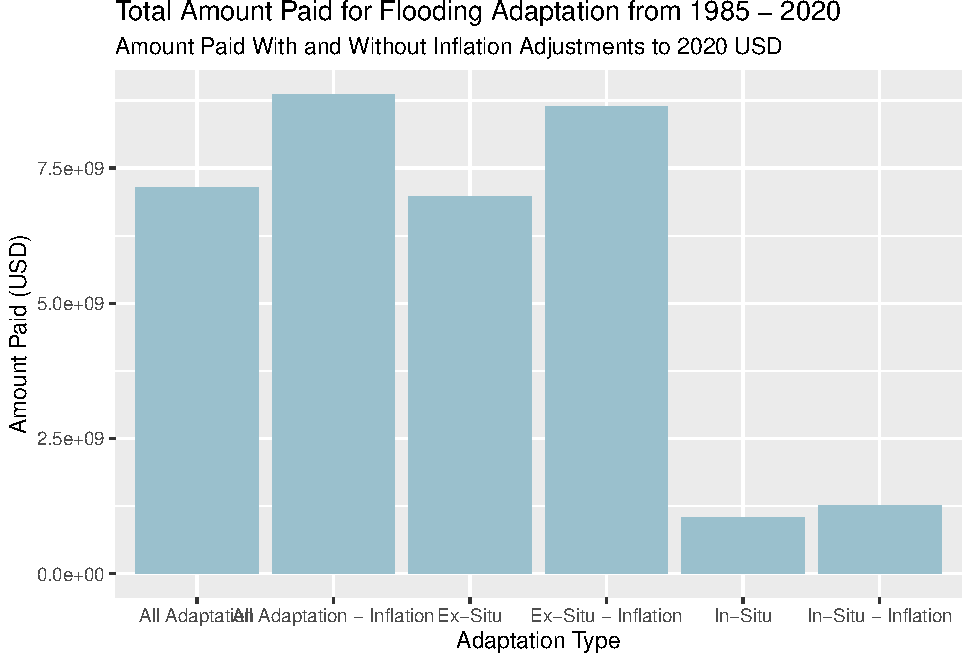
\includegraphics{finalreport_files/figure-latex/unnamed-chunk-2-1.pdf}

Finally, figures 3 and 4 show this same data over time specifically
focusing on the number of properties and total amount paid for all
grants that went towards flooding adaptation. These graphs, as well as
the graphs of ex-situ and in-situ data over time, are further examined
in the analysis section including trendlines to complement the time
series analysis.

\begin{Shaded}
\begin{Highlighting}[]
\FunctionTok{ggplot}\NormalTok{(}\AttributeTok{data =}\NormalTok{ databyyear, }\FunctionTok{aes}\NormalTok{(}\AttributeTok{x =}\NormalTok{ programFy, }\AttributeTok{y =}\NormalTok{ Floodpropertiesperyear)) }\SpecialCharTok{+}
  \FunctionTok{geom\_bar}\NormalTok{(}\AttributeTok{stat =} \StringTok{"identity"}\NormalTok{, }\AttributeTok{fill =} \StringTok{"lightblue4"}\NormalTok{)}\SpecialCharTok{+}
  \FunctionTok{labs}\NormalTok{( }
    \AttributeTok{title =} \StringTok{"Number of Properties that Received Flood Adaptation Grants from 1985 {-} 2020"}\NormalTok{, }
    \AttributeTok{x =} \StringTok{"Year"}\NormalTok{, }
    \AttributeTok{y =} \StringTok{"Number of Properties"}\NormalTok{)}
\end{Highlighting}
\end{Shaded}

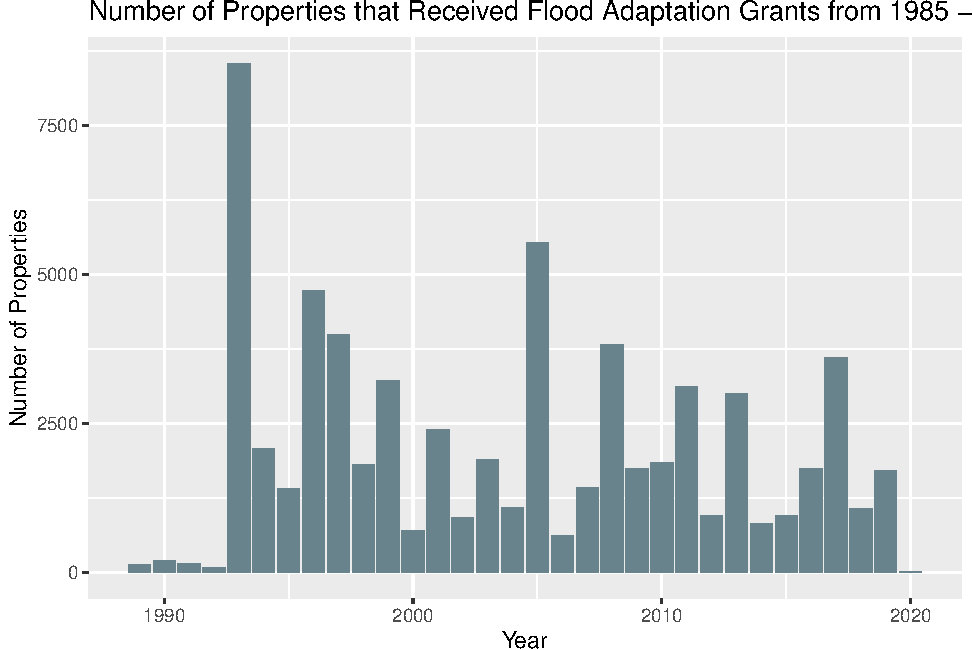
\includegraphics{finalreport_files/figure-latex/unnamed-chunk-3-1.pdf}

\begin{Shaded}
\begin{Highlighting}[]
\FunctionTok{ggplot}\NormalTok{(}\AttributeTok{data =}\NormalTok{ inflation\_data, }\FunctionTok{aes}\NormalTok{(}\AttributeTok{x =}\NormalTok{ programFy, }\AttributeTok{y =}\NormalTok{ InflationAdjusted\_AllAmountpaid)) }\SpecialCharTok{+}
  \FunctionTok{geom\_bar}\NormalTok{(}\AttributeTok{stat =} \StringTok{"identity"}\NormalTok{, }\AttributeTok{fill =} \StringTok{"lightblue3"}\NormalTok{)}\SpecialCharTok{+}
  \FunctionTok{labs}\NormalTok{( }
    \AttributeTok{title =} \StringTok{"Total Amount Paid for Flood Adaptation Grants 1985 {-} 2020"}\NormalTok{, }
    \AttributeTok{x =} \StringTok{"Year"}\NormalTok{, }
    \AttributeTok{y =} \StringTok{"Total Amount Paid (2020 USD)"}\NormalTok{)}
\end{Highlighting}
\end{Shaded}

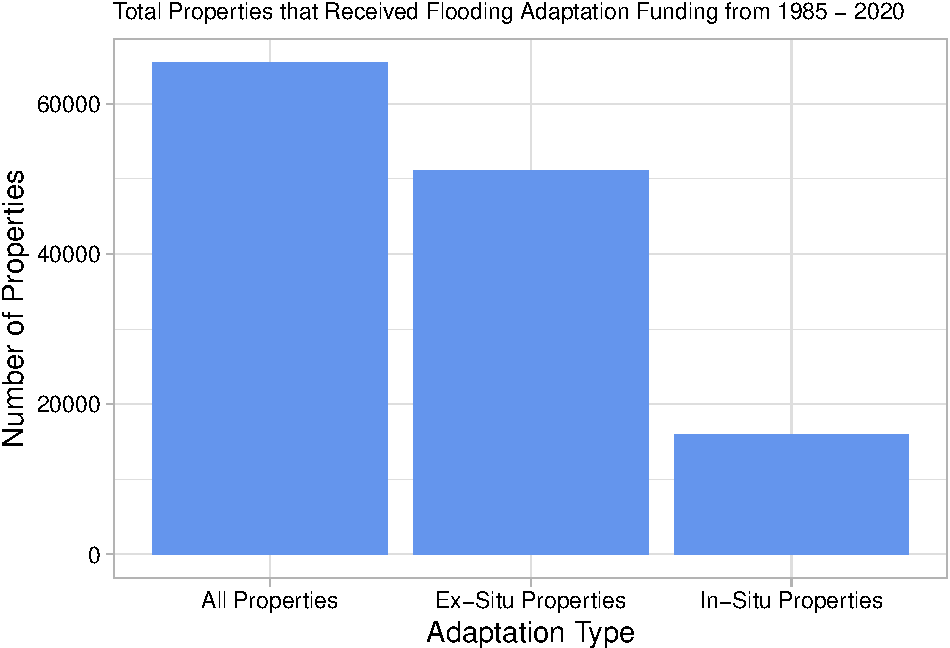
\includegraphics{finalreport_files/figure-latex/unnamed-chunk-4-1.pdf}

\newpage

\hypertarget{analysis}{%
\subsection{Analysis}\label{analysis}}

This analysis involved nine time series analysis that can be understood
based on these more detailed research questions that the time series
helps to answer:

\begin{itemize}
\item
  Total Number of Properties: Is there a monotonic trend in the total
  number of properties that receive grant funding over time?\\
\item
  Total Amount Paid for All Adaptation: Is there a monotonic trend in
  the total amount paid for flooding adaptation grants over time?\\
\item
  Total Amount Paid - Inflation Adjusted: Is there (still) a monotonic
  trend in the total amount paid for flooding adaptation grants over
  time when adjusting for inflation to 2020 dollars?
\item
  Number of Buyouts: Is there a monotonic trend in the total number of
  properties that received ex-situ grant funding, or funding to buyout
  the property, over time?\\
\item
  Amount Paid for Buyouts: Is there a monotonic trend in the amount paid
  for buyouts over time?\\
\item
  Amount Paid for Buyouts - Inflation Adjusted: Is there (still) a
  monotonic trend in the amount paid for buyouts after adjusting for
  inflation to 2020 dollars?
\item
  Number of In-Situ Properties: Is there a monotonic trend in the total
  number of properties that received in-situ grant funding to adapt in
  place over time?\\
\item
  Amount Paid for In-Situ Adaptation: Is there a monotonic trend in the
  amount paid for in-situ adaptation over time?\\
\item
  Amount Paid for In-Situ Adaptation - Inflation Adjusted: Is there
  (still) a monotonic trend in the amount paid for in-situ adaptation
  after adjusting for inflation to 2020 dollars?
\end{itemize}

\hypertarget{question-1-insert-specific-question-here-and-add-additional-subsections-for-additional-questions-below-if-needed}{%
\subsection{Question 1: \textless insert specific question here and add
additional subsections for additional questions below, if
needed\textgreater{}}\label{question-1-insert-specific-question-here-and-add-additional-subsections-for-additional-questions-below-if-needed}}

\hypertarget{question-2}{%
\subsection{Question 2:}\label{question-2}}

\newpage

\hypertarget{summary-and-conclusions}{%
\section{Summary and Conclusions}\label{summary-and-conclusions}}

\newpage

\hypertarget{references}{%
\section{References}\label{references}}

\textless add references here if relevant, otherwise delete this
section\textgreater{}

\end{document}
